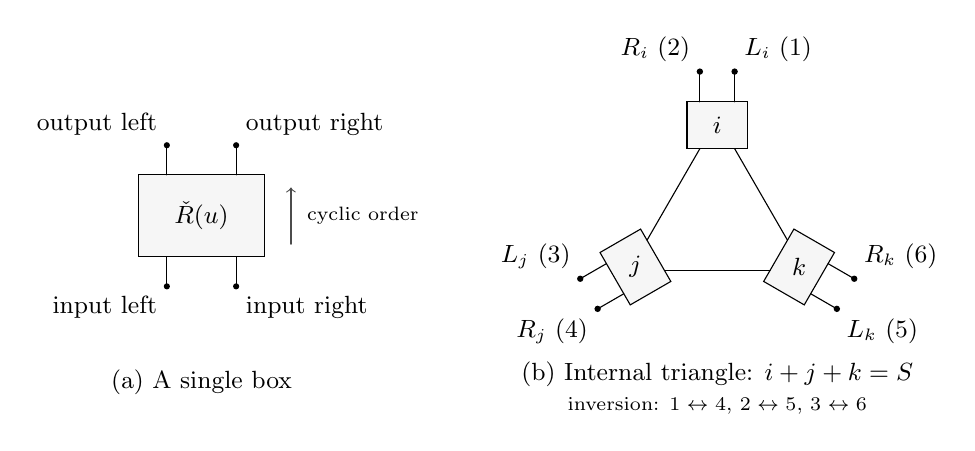
\begin{tikzpicture}[line cap=round,font=\small]
\begin{scope}[xshift=-3.35cm,yshift=.15cm,scale=.8]
\draw[fill=gray!7] (-1,-.65) rectangle (1,.65);
\node at (0,0) {$\check R(u)$};
\foreach \x in {-.55,.55}
  {\draw (\x,-1.12)--(\x,-.65); \draw (\x,.65)--(\x,1.12);}
\fill (-.55,-1.12) circle (1.4pt) node[below left] {input left};
\fill (.55,-1.12) circle (1.4pt) node[below right] {input right};
\fill (.55,1.12) circle (1.4pt) node[above right] {output right};
\fill (-.55,1.12) circle (1.4pt) node[above left] {output left};
\draw[->,black!70] (1.42,-.45)--(1.42,.45);
\node[anchor=west,font=\scriptsize] at (1.52,0) {cyclic order};
\node at (0,-2.65) {(a) A single box};
\end{scope}
\begin{scope}[xshift=3.2cm,yshift=.1cm,scale=.96]
\foreach \ang/\lab in {0/i,120/j,240/k}{
  \begin{scope}[rotate=\ang]
  \draw[fill=gray!7] (-.40,.94) rectangle (.40,1.56);
  \draw (-.23,1.56)--(-.23,1.96);
  \draw (.23,1.56)--(.23,1.96);
  \coordinate (\lab-next) at (-.23,.94);
  \coordinate (\lab-prev) at (.23,.94);
  \coordinate (\lab-L) at (.23,1.96);
  \coordinate (\lab-R) at (-.23,1.96);
  \end{scope}
}
\draw (i-next)--(j-prev);
\draw (j-next)--(k-prev);
\draw (k-next)--(i-prev);
\node at (90:1.25) {$i$};
\node at (210:1.25) {$j$};
\node at (330:1.25) {$k$};
\foreach \lab in {i,j,k}{
  \fill (\lab-L) circle (1.2pt);
  \fill (\lab-R) circle (1.2pt);
}
\node[above right] at (i-L) {$L_i\ (1)$};
\node[above left] at (i-R) {$R_i\ (2)$};
\node[above left] at (j-L) {$L_j\ (3)$};
\node[below left] at (j-R) {$R_j\ (4)$};
\node[below right] at (k-L) {$L_k\ (5)$};
\node[above right] at (k-R) {$R_k\ (6)$};
\node at (0,-2.05) {(b) Internal triangle: $i+j+k=S$};
\node[font=\scriptsize] at (0,-2.46)
  {inversion: $1\leftrightarrow4$, $2\leftrightarrow5$, $3\leftrightarrow6$};
\end{scope}
\end{tikzpicture}
